% ------------------------------------------------------------------------------
% TYPO3 Version 10.4 - What's New (Italian Version)
%
% @license	Creative Commons BY-NC-SA 3.0
% @link		https://typo3.org/help/documentation/whats-new/
% @language	Italian
% ------------------------------------------------------------------------------

\section{Introduzione}
\begin{frame}[fragile]
	\frametitle{Introduzione}

	\begin{center}\huge{Introduzione}\end{center}
	\begin{center}\huge{\color{typo3darkgrey}\textbf{I fatti in breve}}\end{center}

\end{frame}

% ------------------------------------------------------------------------------
% TYPO3 Version 10.4 - The Facts

\begin{frame}[fragile]
	\frametitle{Introduzione}
	\framesubtitle{TYPO3 Versione 10.4 - I fatti in breve}

	\begin{itemize}
		\item Data di rilascio: 21 Aprile 2020
		\item Tipo di rilascio: LTS (Long-term Support)
	\end{itemize}

	\begin{figure}
		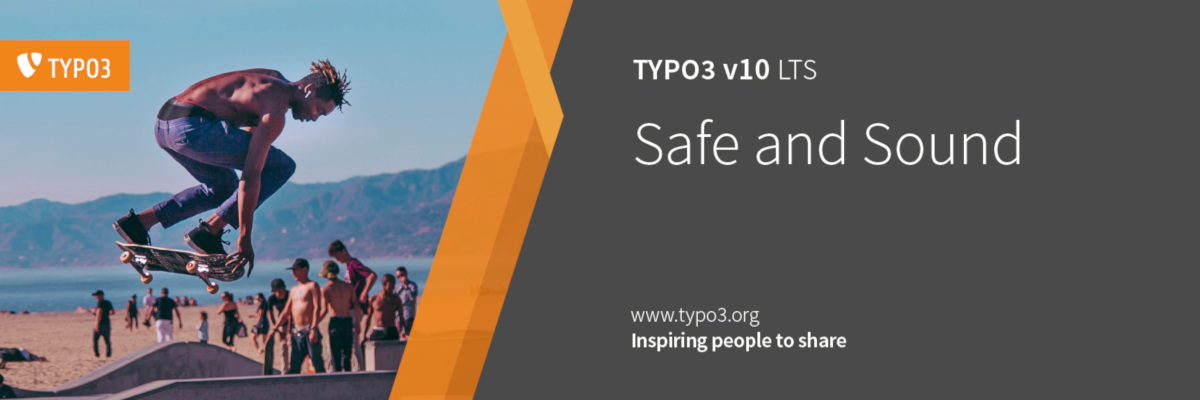
\includegraphics[width=0.95\linewidth]{Introduction/typo3-v10-4-banner.jpg}
	\end{figure}

\end{frame}

% ------------------------------------------------------------------------------
% TYPO3 Version 10.4 - Executive Summary

\begin{frame}[fragile]
	\frametitle{Introduzione}
	\framesubtitle{Sintesi}

	\small
		TYPO3 v10.4 (chiamato anche TYPO3 v10 LTS indicando che si tratta di una versione di supporto
		a lungo termine) è la nostra nuova ammiraglia e, senza dubbio, uno dei sistemi di gestione dei
		contenuti open source basati su PHP più avanzati attualmente sul mercato.

		\vspace{0.2cm}

		Dopo aver pubblicato cinque versioni di sprint da luglio 2019, possiamo affermare con orgoglio
		che abbiamo dotato TYPO3 delle migliori librerie PHP moderne e che abbiamo introdotto alcune
		fantastiche nuove funzionalità aziendali.

		\vspace{0.2cm}

		Si noti che questo documento riepiloga solo le modifiche tra TYPO3 v10.3 e v10.4.

		\vspace{0.2cm}

		"What's New Slides" di tutte le versioni TYPO3 v10.x sono disponibili all'indirizzo
		\href{https://typo3.org/help/documentation/whats-new/}{typo3.org}.

	\normalsize

\end{frame}

% ------------------------------------------------------------------------------
% System Requirements

\begin{frame}[fragile]
	\frametitle{Introduzione}
	\framesubtitle{Requisiti di sistema}

	\begin{itemize}
		\item PHP versione 7.2, 7.3 or 7.4
		\item Impostazioni PHP:

			\begin{itemize}
				\item \texttt{memory\_limit} >= 256M
				\item \texttt{max\_execution\_time} >= 240s
				\item \texttt{max\_input\_vars} >= 1500
				\item l'opzione di compilazione \texttt{-}\texttt{-disable-ipv6} \underline{non} deve essere usata
			\end{itemize}

		\item La maggior parte dei database supportati da \textbf{Doctrine DBAL} funzionano anche con TYPO3.
			I DB verificati sono ad esempio:
	\end{itemize}

	\begin{figure}
		
\includegraphics[width=0.80\linewidth]{Introduction/logo-databases.png}
	\end{figure}

\end{frame}

% ------------------------------------------------------------------------------
% Development, Release, and Maintenance Timeline

\begin{frame}[fragile]
	\frametitle{Introduzione}
	\framesubtitle{Sviluppo, tempi di rilascio e mantenimento}

	\textbf{TYPO3 v10}

	\begin{figure}
		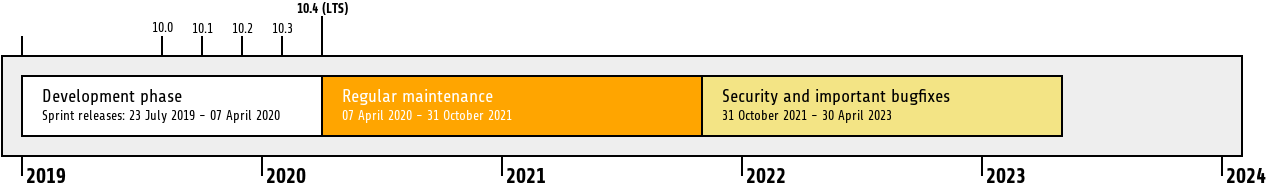
\includegraphics[width=1\linewidth]{Introduction/typo3-v10-lifecycle.png}
	\end{figure}

	\textbf{Supporto esteso}\newline
	\smaller
		La \href{https://typo3.com}{TYPO3 GmbH} offre ulteriori opzioni di supporto
		per TYPO3 v10 LTS anche dopo il 30 Aprile 2023, per ulteriori due anni.
	\normalsize

\end{frame}

% ------------------------------------------------------------------------------
% TYPO3 v10 Roadmap

\begin{frame}[fragile]
	\frametitle{Introduzione}
	\framesubtitle{TYPO3 v10 Roadmap}

	Date di rilascio e loro obiettivi principali:

	\begin{itemize}

		\item v10.0 \tabto{1.1cm}23/Lug/2019\tabto{3.4cm}Preparare la strada per nuovi concetti e API entusiasmanti
		\item v10.1 \tabto{1.1cm}01/Ott/2019\tabto{3.4cm}Miglioramenti nel routing e nel gestore di sito v2
		\item v10.2 \tabto{1.1cm}03/Dic/2019\tabto{3.4cm}Miglioramenti al motore di rendering Fluid
		\item v10.3 \tabto{1.1cm}25/Feb/2020\tabto{3.4cm}Conferma della funzionalità
		\item
			\begingroup
				\color{typo3orange}
				v10.4 \tabto{1.1cm}21/Apr/2020\tabto{3.4cm}Rilascio LTS (Long-term Support)
			\endgroup

	\end{itemize}

	\vspace{0.6cm}
	\smaller
		\url{https://typo3.org/article/typo3-v10-roadmap}\newline
		\url{https://typo3.org/article/typo3-v10-lts-safe-and-sound}
	\normalsize

\end{frame}

% ------------------------------------------------------------------------------
% Installation

\begin{frame}[fragile]
	\frametitle{Introduzione}
	\framesubtitle{Installazione}

	\begin{itemize}
		\item Procedura ufficiale, \textit{classica}, di installazione in Linux/Mac OS X\newline
			(Directory Root ad esempio \texttt{/var/www/site/htdocs}):
\begin{lstlisting}
$ cd /var/www/site
$ wget --content-disposition get.typo3.org/10.4
$ tar xzf typo3_src-10.4.0.tar.gz
$ cd htdocs
$ ln -s ../typo3_src-10.4.0 typo3_src
$ ln -s typo3_src/index.php
$ ln -s typo3_src/typo3
$ touch FIRST_INSTALL
\end{lstlisting}

		\item Link simbolici in Microsoft Windows:

			\begin{itemize}
				\item Usa \texttt{junction} in Windows XP/2000
				\item Usa \texttt{mklink} in Windows Vista e Windows 7 e superiori
			\end{itemize}

	\end{itemize}
\end{frame}

% ------------------------------------------------------------------------------
% Installation using composer

\begin{frame}[fragile]
	\frametitle{Installazione e aggiornamento}
	\framesubtitle{Installazione con \texttt{composer}}

	\begin{itemize}
		\item Installazione con \textit{composer} in Linux, Mac OS X e Windows 10:
\begin{lstlisting}
$ cd /var/www/site/
$ composer create-project typo3/cms-base-distribution typo3v10 ^10.4
\end{lstlisting}

		\item In alternativa, crea il tuo file \texttt{composer.json} ed esegui:
\begin{lstlisting}
$ composer install
\end{lstlisting}

			Maggiori informazioni e un esempio di file \texttt{composer.json} sono disponibili su:\newline

			\small
				\href{https://get.typo3.org/misc/composer/repository}{https://get.typo3.org/misc/composer/repository}
			\normalsize

	\end{itemize}
\end{frame}

% ------------------------------------------------------------------------------
